
In this section, our primary goal is to preprocess the data effectively to ensure it is ready for machine learning algorithms and free from errors. By the end of this exploration and analysis, the dataset should be clean and well-prepared for model training. We will address the following key criteria:

\begin{enumerate}
    \item \textbf{Presence of Missing Values:} The dataset is checked for presence of any missing values. Null values can complicate numerical computations and degrade model performance. To address this, we will either impute missing values or remove the affected rows/columns to maintain data integrity.

    \item \textbf{Check for Duplicates:} Duplicate samples with identical characteristics can skew the results and reduce model performance. We will identify and remove any duplicate entries to ensure each sample in the dataset is unique.

    \item \textbf{Feature Selection:} Selecting the most informative features is undeniably one of the most important tasks before feeding the data into machine learning models. In this particular dataset, since we do not have prior knowledge about the information provided by features, we will only rely on the identification of correlation among features, to filter our highly correlated features.

    \item \textbf{Feature Normalization:} In the data exploration step, we discovered that the features in our dataset vary in range, which can negatively impact the performance of certain algorithms such as SVM. Therefore, we need to adopt normalization techniques to prevent side effects, ensuring they contribute equally to the model's learning process.

    \item \textbf{Partitioning the Dataset:} To prevent data leakage and ensure a fair evaluation of our models, we will split the dataset into training and test sets. This separation ensures that the test set remains unseen during training, providing an unbiased assessment of model performance and ensuring that we follow a sound methodology.
\end{enumerate}

% ------------------------------------------------------
\section{Presence of Missing Values}

As we mentioned earlier in the previous section, there is no Null values present in our dataset, hence no further consideration is required in this regard.

However, in order to confirm this and analyze the existence of Null values, we will count the occurrences of such values using \texttt{isnull()} function in each column. It was confirmed that all the columns were free of missing values.

% ------------------------------------------------------
\section{Check for Duplicates}

Using the \texttt{duplicated} function provided by Pandas, we can count the duplicated rows. As it turns out, there are no duplicated rows present in our dataset, therefore no actions are expected in this manner.

% ------------------------------------------------------
\section{Feature Selection}

It is evident that many of the machine learning applications rely on the fact the features are \textit{independent} from each other, hence they are not correlated with one another. Highly correlated features can sometimes provide redundant information, where we might consider dimensionality reduction techniques or feature selection methods in such cases.

The identification of the correlation among features is an important task, which can be achieved by using the \textit{correlation matrix} to assess the correlation among different features and identify potentially irrelevant information. A correlation matrix provides the correlation coefficients between pairs of features, which helps to understand the relationships between them. After computing this matrix, we attempt to visualize it using a \textit{heatmap} to analyze the situation appropriately.

\begin{figure}[h]
    \centering
    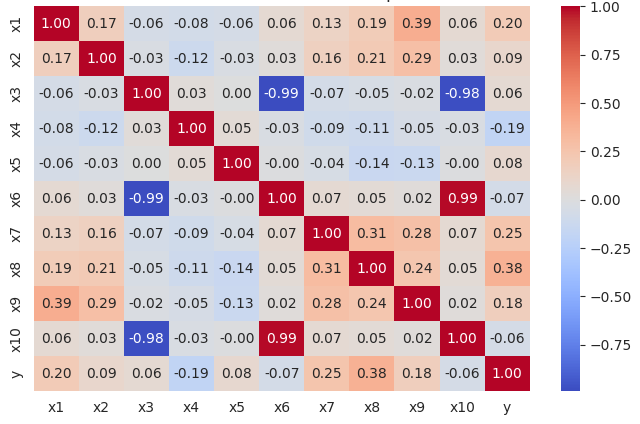
\includegraphics[width=0.8\linewidth]{images/correlation.png}
    \caption{Correlation Matrix Heatmap}
    \label{fig:correlation}
\end{figure}

Interpreting the correlation matrix:
\begin{itemize}
    \item The "red" cells with values close to \texttt{1} denote perfect positive correlation
    \item The "blue" cells with values close to \texttt{-1} denote perfect negative correlation
    \item The "light" cells with values close to \texttt{0} denote no correlation among those features
\end{itemize}

Analyzing the correlations, it can be seen that the features $x_6$ and $x_{10}$ are positively correlated together (with value \texttt{0.99}) while being negatively correlated with $x_3$ (with values \texttt{-0.99} and \texttt{-0.98}). Additionally, analyzing their correlation with respect to the label $y$, it can be seen that all of them similarly hold a value close to \texttt{0.06}, providing no extra information compared to the other one for the classification.

After identifying highly correlated features, since we have a few number of features available, we will proceed with manually removing redundant features that are highly correlated. To this regard, we remove the features $x_3$ and $x_{10}$, preserving the feature $x_6$ in our dataset.

% ------------------------------------------------------
\section{Feature Normalization}

The two most common techniques for normalization are:
\begin{itemize}
    \item \textbf{Min-Max Scaling}, which scales the data to a fixed range (usually \texttt{0} to \texttt{1}).
    \item \textbf{Z-score Normalization}, which standardizes the features to have a mean of \texttt{0} and a standard deviation of \texttt{1}.
\end{itemize}


The \textit{Z-score Normalization} technique is more consistent with respect to Gaussian assumptions, and it is more reliable when dealing with algorithms that assume normal distribution centered around zero. Therefore, it naturally fits better our problem, and we will proceed with this technique. It can be computed as:

\begin{equation}
    Z = \frac{X-\mu}{\sigma}
\end{equation}

where $X$ represents each feature, and the corresponding mean and standard deviation for each of the features are $\mu$ and $\sigma$, respectively.

% ------------------------------------------------------
\section{Partitioning the Dataset}

To maintain the integrity of our data and prevent data leakage, one approach is to partition the dataset into training and test sets, such that the model is trained on the training set and its performance is evaluated on the test set. This partitioning can be achieved as follows:

\begin{enumerate}
    \item \textbf{Shuffle the Data:} The dataset is shuffled to randomize the order of the samples, ensuring a more representative distribution and reducing the likelihood of biased results due to any inherent order in the data.
    \item \textbf{Split the Data:} The shuffled data is partitioned such that the first \texttt{80\%} of the samples are allocated to the training set, while the remaining \texttt{20\%} are reserved for the test set.
    \item \textbf{Separate Features and Labels:} The target labels are separated from the feature variables, being stored in variables $X$ (features) and $y$ (labels) for both training and test sets.
\end{enumerate}

This procedure ensures that the training and test sets are appropriately isolated, preserving the validity of our model evaluation.

However, since we aim to perform hyper-parameter optimization alongside our model implementation, we will adopt the \textit{K-Fold Nested Cross-Validation} technique instead, which is fully discussed in the next section.